\usepackage{svg}

\definecolor{codegreen}{rgb}{0,0.6,0}
\definecolor{codegray}{rgb}{0.5,0.5,0.5}
\definecolor{codepurple}{rgb}{0.58,0,0.82}
\definecolor{backcolour}{rgb}{0.95,0.95,0.92}

\lstdefinelanguage{Godot}{
	keywords={class_name, func, for, return, in range, is, var, not, continue, or},
	morecomment=[l]{#}
}

\lstdefinelanguage{Pseudo}{
	keywords={FUNCTION, IMPORT, END if, then, void},
	morecomment=[l]{//}
}

\lstdefinelanguage{dict}{
	keywords={class_name, func, for, return, in range, is, var, not, continue},
}

\lstdefinestyle{mystyle}{
    backgroundcolor=\color{backcolour},   
    commentstyle=\color{codegreen},
    keywordstyle=\color{magenta},
    numberstyle=\tiny\color{codegray},
    stringstyle=\color{codepurple},
    basicstyle=\ttfamily\footnotesize,
    breakatwhitespace=false,         
    breaklines=true,                 
    captionpos=b,                    
    keepspaces=true,                 
    numbers=left,                    
    numbersep=5pt,                  
    showspaces=false,                
    showstringspaces=false,
    showtabs=false,                  
    tabsize=2
}

\lstset{style=mystyle}


\chapter{Implementierung des Lösungskonzepts}
\label{chap:implementierung lk}

Die praktische Umsetzung des GOAP Systems wird nun in diesem Kapitel beschrieben. Es soll insbesondere auf die Umsetzung des GOAP-Entscheidungssystem eingegangen werden. Zunächst wird die grundlegende Architektur von GOAP mit ihren Modulen erläutert, gefolgt von einer Darstellung des Szenarios, in dem die \hyperref[chap:entscheidungssysteme]{Entscheidungssysteme} implementiert werden. Abschließend wird die Realisierung der Benchmarks behandelt.

So soll die Grundlegende GOAP Architektur anhand von UML-Notation dargestellt und beschrieben werden. Sie bildet die Grundlage für die Implementation des Entscheidungssystems im Szenario. Mithilfe von Pseudocode werden die in den UML-Klassendiagrammen dargestellten Methoden und Attribute weiter erläutert. Die Architektur basiert dabei auf den Informationen aus dem GOAP Grundkapitel\ref{}, wissenschaftlicher Literatur zum Thema GOAP und der F.E.A.R SDK\autocite{}.

\section{GOAP Architektur}
\label{chap:goap architektur}

Aus dem GOAP-Kapitel\ref{} geht hervor, dass ein GOAP-System aus einem Planner, Zielen, Aktionen und einer FSM besteht. Diese Module sollen ihre Aufgaben erfüllen, wie im Grundlagenkapitel zu GOAP beschrieben. Dafür müssen diese Module in einer Architektur zusammenarbeiten. Die grundlegende Architektur von GOAP wird in Abbildung\ref{} dargestellt.

Der Agent wird über eine GoapAgent Klasse realisiert. Sie soll in der Architektur die Hauptklasse darstellen und als Schnittstelle zur restlichen Spielwelt fungieren. Die Spielwelt benötigt nämlich eine Schnittstelle, um dem NPC Informationen zu übergeben, wie beispielsweise bestimmte Koordinaten zum erfüllen bestimmter Aktionen. Die zentrale Aufgabe des GoapAgent ist nämlich die Aktionen einer Aktionssequenz ausführen. Für die Ausführung der eigentlichen Aktionen werden dabei \hyperref[chap:game-objects]{Komponenten} benötigt, welche die Spielwelt manipulieren können. Die Klasse Npc\ref{} stellt diese Komponenten bereit. Ein Beispiel einer solchen Komponente ist die vision\_component, die es dem NPC ermöglicht den Spieler zu erfassen.

Der StateManager verwaltet die Zustände des NPC, die von GoapAction und GoapGoal abgefragt werden. Diese Zustände können über die Komponenten der Oberklasse Npc oder durch nichtdeterministische Umstände der Spielwelt verändert werden. Ein Beispiel für einen Zustand der im StateManager verwaltet wird, ist die Sichtbarkeit der Spielfigur, die durch die vision\_component beeinflusst wird.

Für die Generierung von Aktionssequenzen des GoapAgent ist die Klasse GoapPlanner zuständig. Wie in der Architektur dargestellt, besitzt der GoapPlanner Objekte der Klassen GoapGoal, GoapAction und AStarNode, welche dazu benötigt werden eine Aktionssequenz zu finden. Aus den GoapGoal Objekten wählt der GoapPlanner einen Zielzustand aus, für den eine Aktionssequenz gesucht wird. Der GoapPlanner sucht die Aktionssequenz mithilfe des A$^*$ Algorithmus\ref{}. Die Klasse AStarNode wird zur Generierung von Knoten für den Suchbaum des A$^*$ Algorithmus benötigt. Ein AStarNode setzt dabei die Eigenschaften eines Suchbaum-Knoten\ref{} um.

Die Klasse GoapAction stellt die Basisklasse für Aktionen dar. Eine Aktion repräsentiert dabei eine Kante im Suchbaum\ref{}.

Es wird keine FSM in der Architektur umgesetzt, da die Implementation keine Animationen umfasst. Stattdessen geschieht die Ausführung der Aktionen direkt innerhalb der Klasse GoapAgent. Sollten Animationen vorhanden sein, können diese auch über die Klasse GoapAction ausgeführt werden. Es besteht keine zwingende Notwendigkeit, eine FSM innerhalb von GOAP umzusetzen. Ein Konzept für die Implementierung einer FSM wäre es, diese an den GoapAgent oder GoapPlanner zu koppeln und die Aktionssequenz von dort aus auszuführen. Die Aktionen würden dann auch die Knotenwechsel für die FSM durchführen.

\begin{figure}[h]
  \centering
  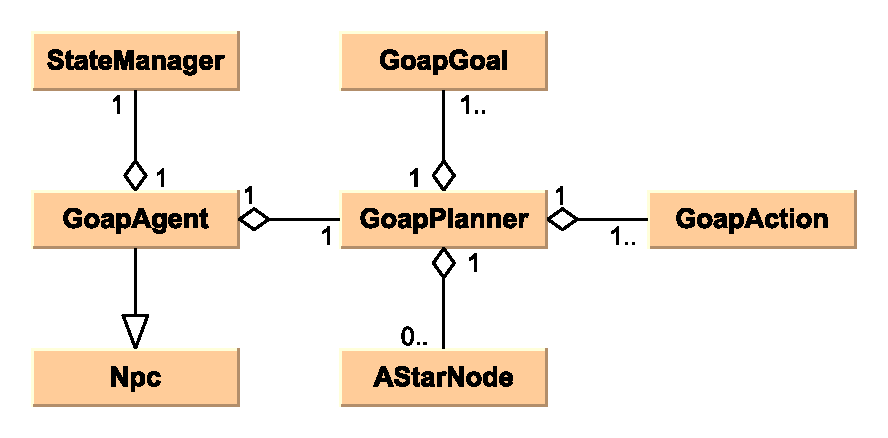
\includegraphics[width=0.8\textwidth, trim=20 20 20 20]{Implementation/goap arc.pdf}
	\captionsetup{justification=justified, format=plain}
  \caption{GOAP Architektur}
  \label{fig:GOAP Architektur}
\end{figure}

\subsection{GoapAgent}
\label{chap:goapagent uml}

Die Abbildung\ref{} stellt die Klasse GoapAgent dar. In den folgenden Unterkapiteln werden die Klassenattribute und Methoden in ihrer Funktion beschrieben. Der GoapAgent speichert folgende Klassenvariablen: goap\_planner, action\_sequence und den current\_step. Bei den Methoden handelt es sich um: update und follow\_sequence.

\subsubsection{Klassenatribute}
\label{chap:goapagent klassenatribute}

Der goap\_planner ist eine Referenz auf die Klasse GoapPlanner, welcher die action\_sequence des GoapAgent bestimmt. Das Array action\_sequence speichert Objekte vom Typ der Klasse GoapAction. Sie stellt die ermittelte Aktionssequenz durch den A* Algorithmus dar. Die Integer-Klassenvaraible current\_step handelt als Indexzeiger, welcher auf die aktuell auszuführende Aktion des action\_sequence verweist.

% Goap Agent
\begin{figure}[h]
  \centering
  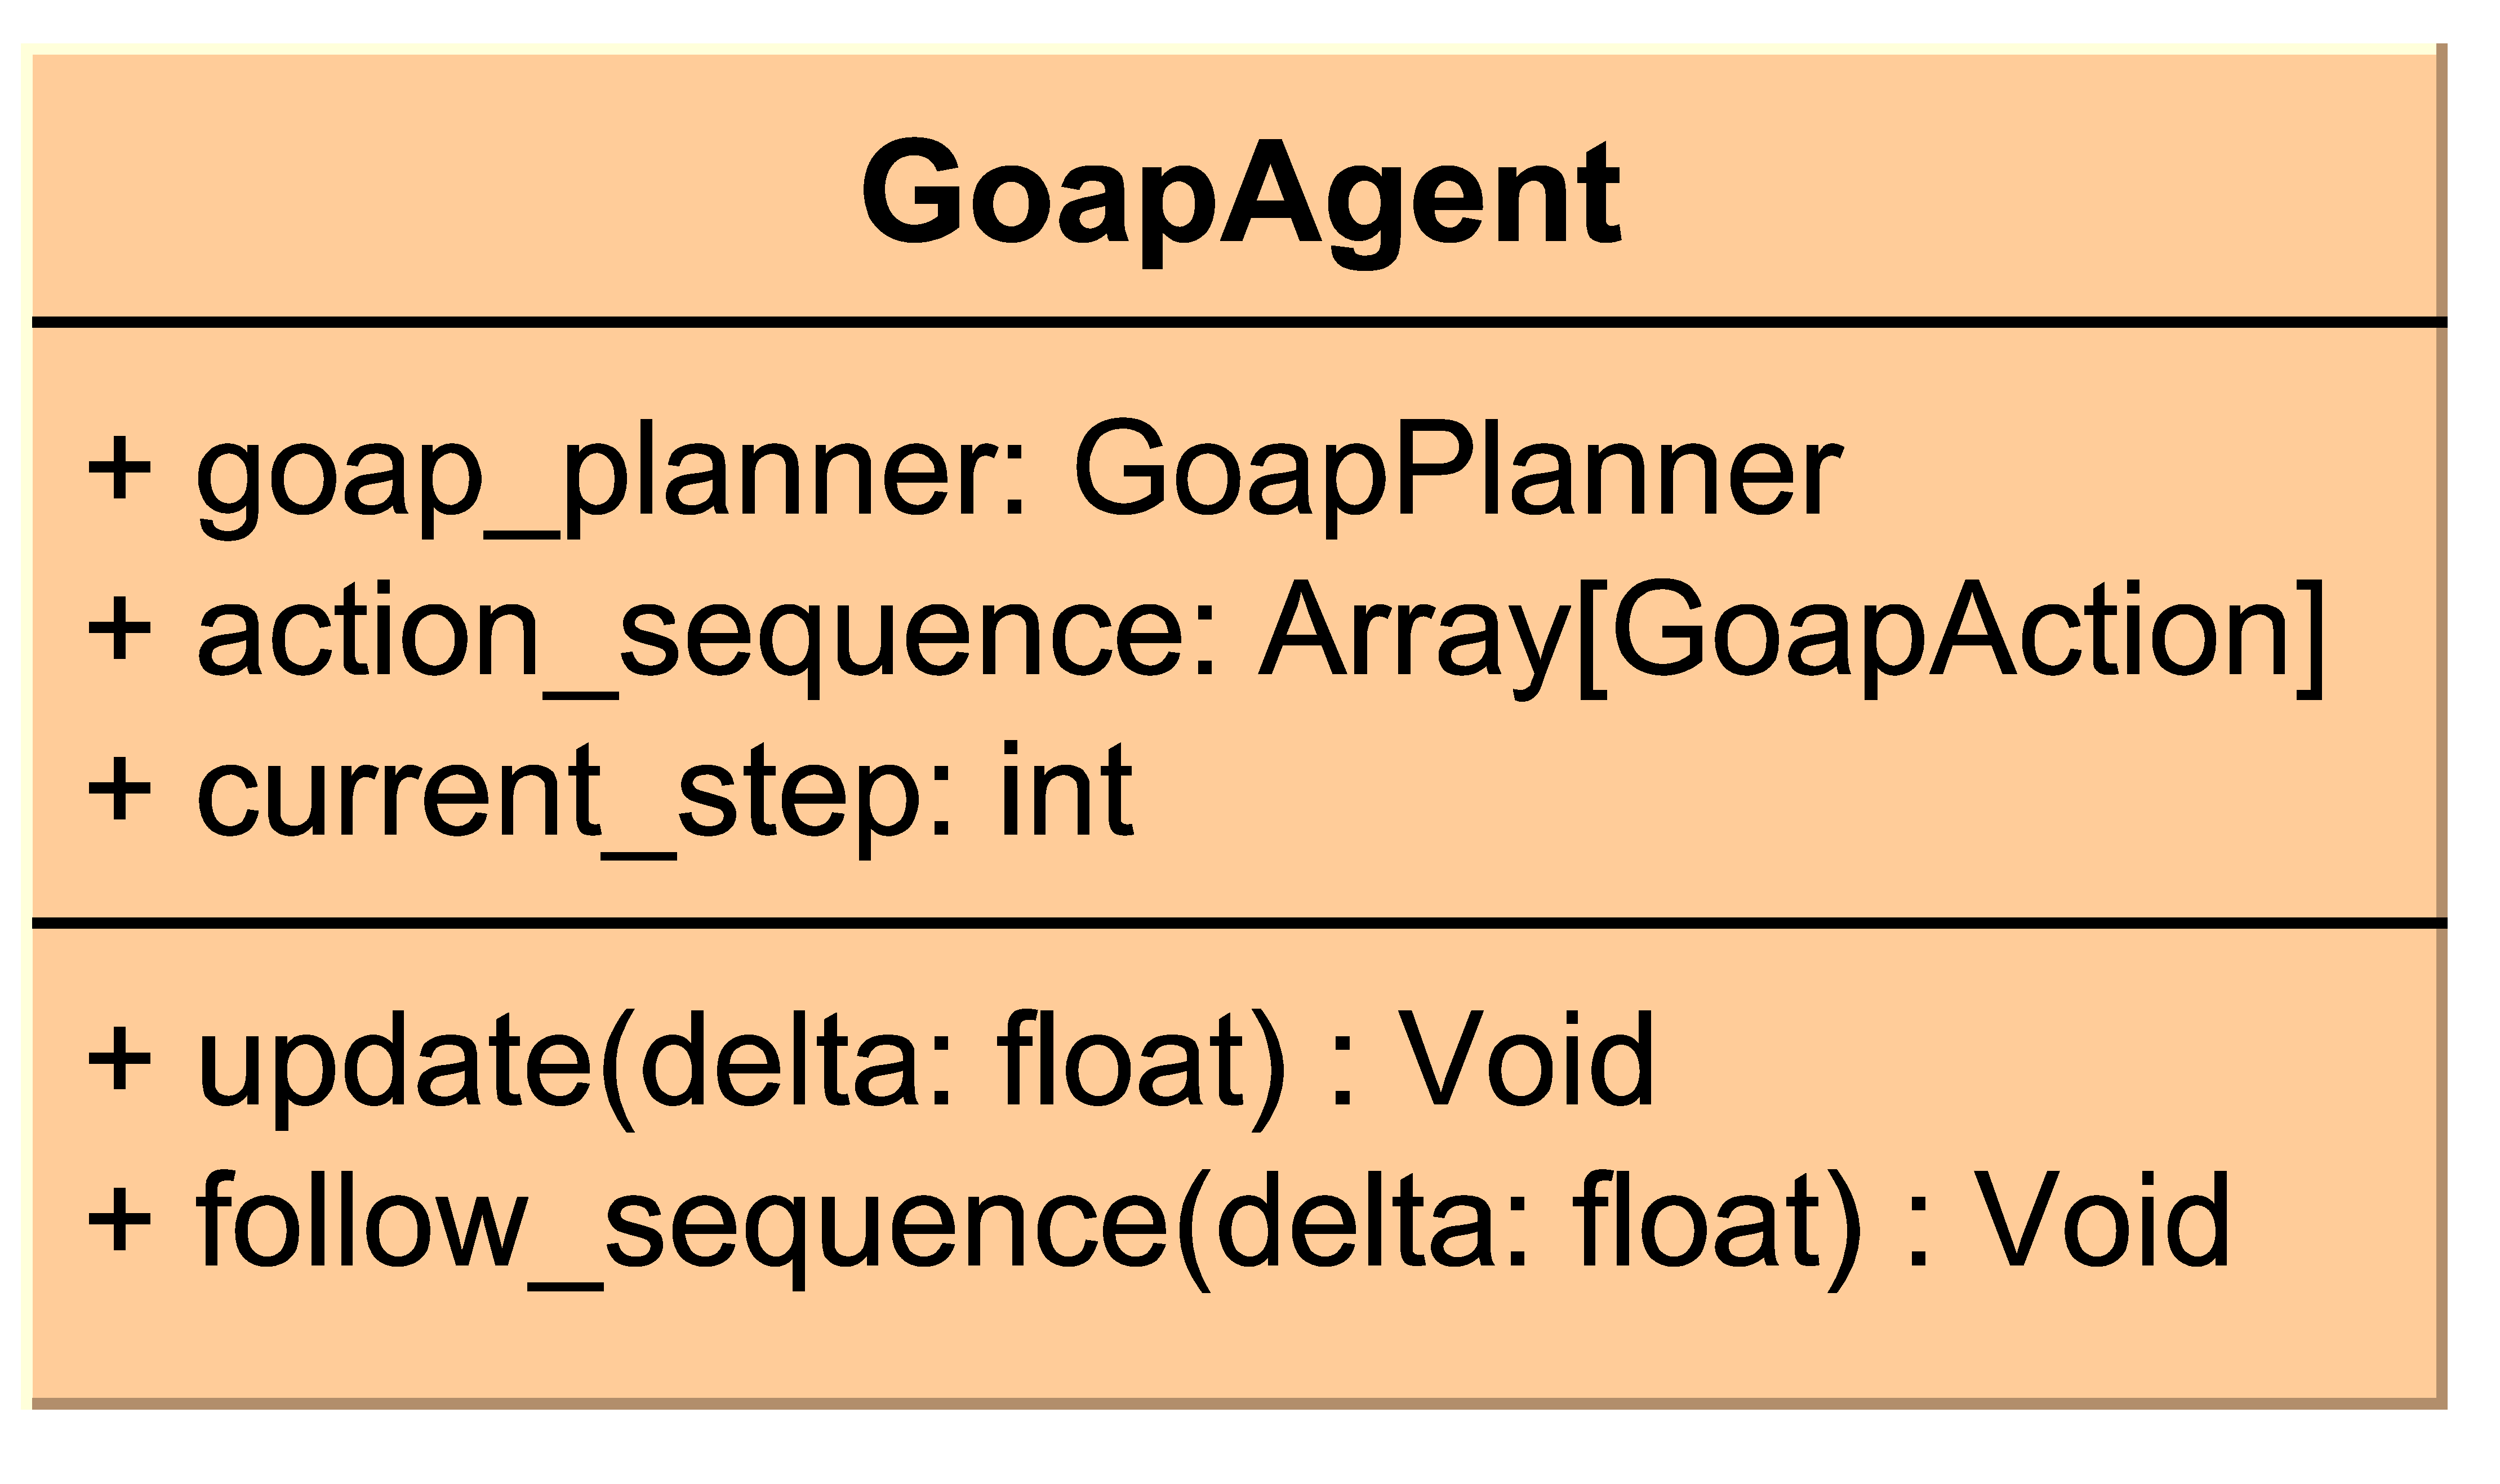
\includegraphics[width=0.5\textwidth]{Lösungskonzept/agent.pdf}
	\captionsetup{justification=justified, format=plain}
  \caption{GoapAgent}
  \label{fig:GoapAgent}
\end{figure}

\subsubsection{Methoden}
\label{chap:goapagent methoden}

Die update Methode ruft Methoden der Klassen und \hyperref[chap:game-objects]{Komponenten} innerhalb des NPC auf. Sie wird wiederum durch eine \_process Funktion jedes \textit{Frame} aufgerufen, um kontinuierliche Logik wie Bewegungen oder Raycasting des GoapAgent zu verarbeiten. Sie wird über die Komponente aufgerufen, welche das Objekt GoapAgent instanziiert. Der Parameter delta repräsentiert die Zeit seit dem letzten Frame und könnte an andere Methoden übergeben werden.

% update Methode
%\lstinputlisting[firstline=0, language=Pseudo, linerange={1-7}, caption={update Methode des GoapAgent}, label=lst:caption]{code/goap agent.txt}

\begin{lstlisting}[language=Pseudo, caption={update Methode des GoapAgent}, mathescape=true]
FUNKTION update(delta) $\rightarrow$ void
    WENN goap_planner neue action_sequence gefunden hat DANN
        current_step $\leftarrow$ 0
        action_sequence $\leftarrow$ goap_planner.get_current_sequence()
    ENDE WENN
    follow_sequence(delta)
ENDE update()
\end{lstlisting}

In der update Methode werden Abfragen gestellt, ob der goap\_planner eine neue action\_sequence generiert hat. Wurde eine neue action\_sequence generiert, so wird die Objektvariable current\_step auf $0$ zurückgesetzt und die neue action\_sequence aus dem goap\_planner abgerufen. Die action\_sequence wird darauf durch die Methode follow\_sequence ausgeführt werden.

% follow_sequence Methode
Über die Methode follow\_sequence geschieht die eigentliche Ausführung der Aktionen aus der action\_sequence. Sollte action\_sequence leer sein, bereits ausgeführt worden oder ungültig sein, so wird eine neue action\_sequence von dem goap\_planner gefordert werden. Ansonsten wird mithilfe des current\_step Index die jeweilige Aktion über ihre GoapAction update Methode ausgeführt werden. Bei erfolgreicher Ausführung der Aktion wird der current\_step inkrementiert, um auf die nächste Aktion der action\_seqeunce zugreifen zu können.

\begin{lstlisting}[language=Pseudo, caption={follow\_sequence Methode des GoapAgent}, mathescape=true]
FUNKTION follow_sequence(delta) : void
	WENN action_sequence leer ODER action_sequence durchgegangen ODER action_sequence[current_step] DANN
		goap_planner.set_create_sequence(WAHR)
		ENDE FUNKTION
	ENDE WENN
	WENN action_sequence[current_step].update(delta) ausgeführt DANN
		current_step um 1 erhöhen
	ENDE WENN
ENDE FUNKTION
\end{lstlisting}




\subsection{GoapPlanner}
\label{chap:goapplanner uml}

Die Abbildung\ref{} zeigt den Aufbau des GoapPlanner. Bei den Methoden handelt es sich um: 

\begin{figure}[h]
  \centering
  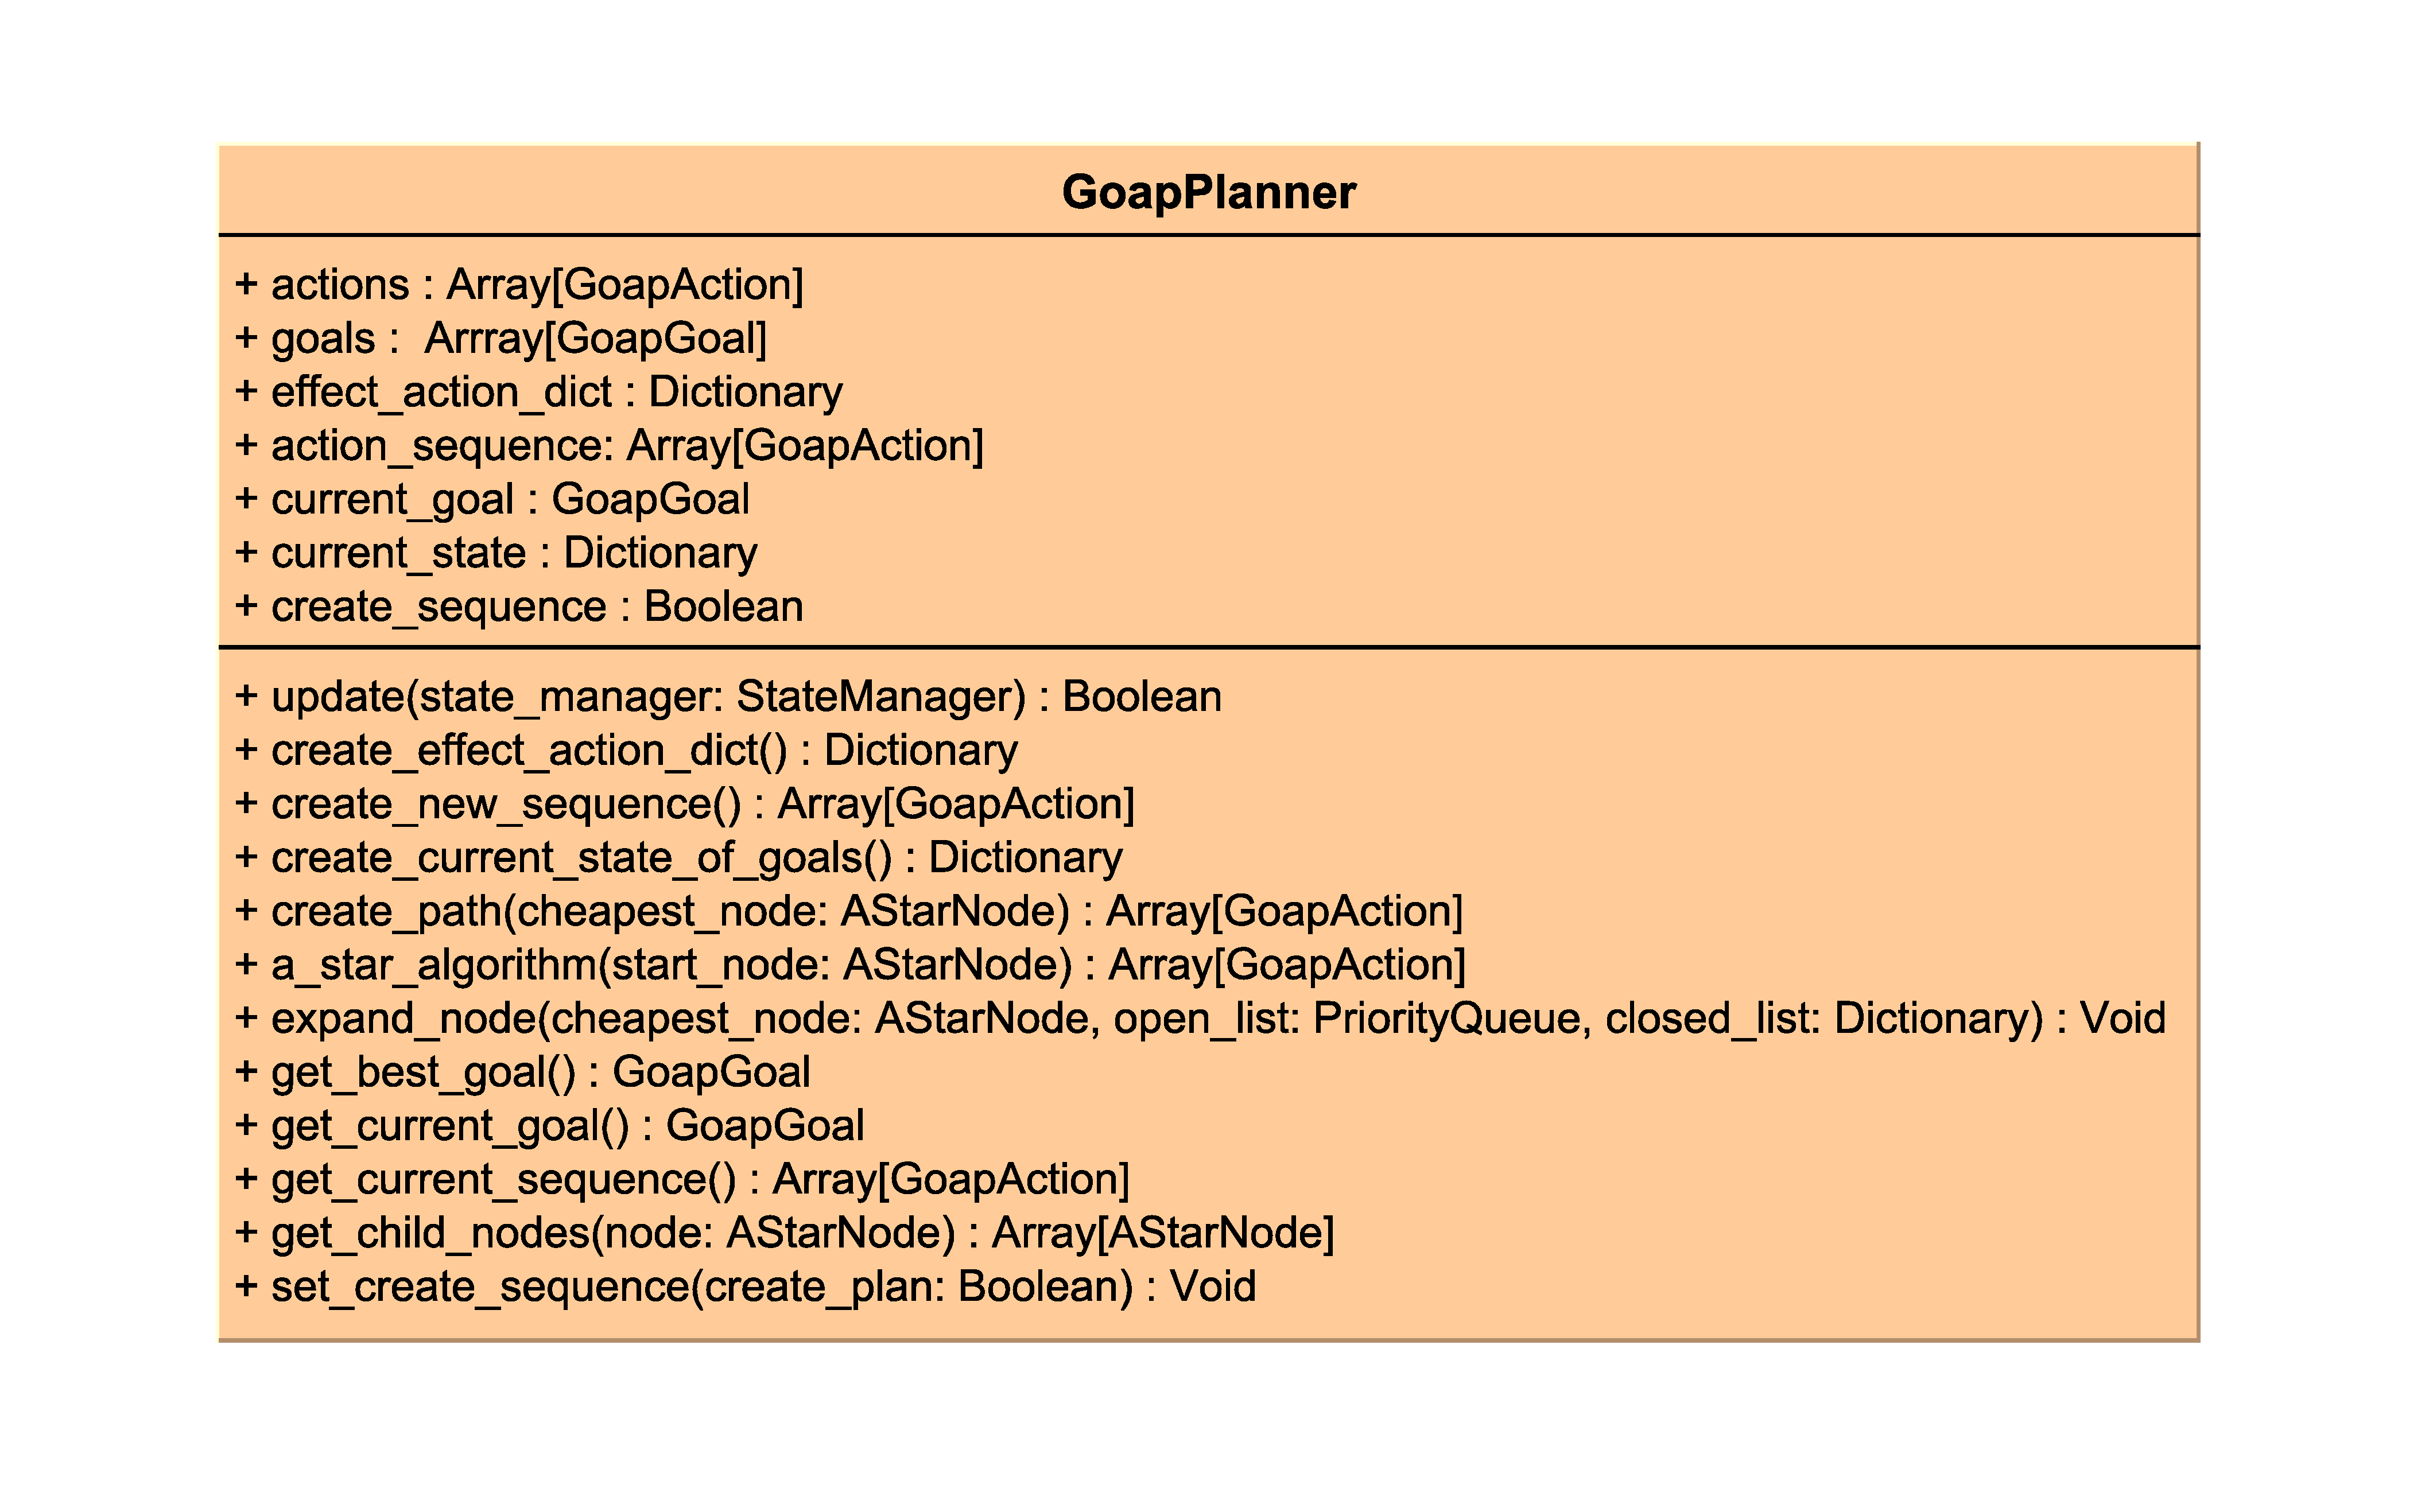
\includegraphics[width=\textwidth, trim=20 20 20 20]{Lösungskonzept/planner.pdf}
	\captionsetup{justification=justified, format=plain}
  \caption{GoapPlanner}
  \label{fig:GoapPlanner}
\end{figure}

\subsubsection{Klassenatribute}
\label{chap:goapplanner klassenattribute}

Der GoapPlanner arbeitet mit Zielen und Aktionen, welche durch die Arrays actions und goals gegeben werden. Über current\_goal wird das Ziel gespeichert, zu dem eine action\_sequence gesucht wird. Die action\_sequence ist die generierte Aktionssequenz durch den GoapPlanner und wird in einem Array mit GoapAction als Elementtyp gespeichert. Das current\_state Dictionary speichert den derzeitigen Zustand des NPC. Die Initialisierung des current\_state findet über den state\_manager Parameter statt, welcher über die update Methode übergeben wird. Das create\_sequence Attribut informiert den GoapPlanner darüber, ob eine neue action\_sequence generiert werden soll. Das effect\_action\_dict Dictionary speichert alle Zustände als \textit{key} und die Aktionen, welche den Zustand beeinflussen können als \textit{values}. So erhält man eine schnellere Zugriffszeit, als wenn man jeden Effekt einer Aktion im Array mit dem benötigten Zustand vergleicht. Ähnlich zur Tabelle, wie im GOAP Grundlagenkapitel \ref{}.

%\begin{lstlisting}[language=dict, caption={effect\_action\_dict aus der Implementierung}]
%effect_action_dict = {
    %"player_eliminated": [
        %RangedAttackFromCover:<Node#82829117475>,
        %MeleeAttack:<Node#82845894692>,
        %RangedAttack:<Node#82812340258>
    %],
    %"player_block_visited": [
        %GoToNode:<Node#82862671909>
    %],
    %"at_patrol_node": [
        %GoToNode:<Node#82862671909>
    %],
    %"at_cover_node": [
        %GoToNode:<Node#82862671909>
    %],
    %"bullets": [
        %Reload:<Node#82879449126>
    %]
%}
%\end{lstlisting}

\subsubsection{Methoden}
\label{chap:goapplaner methoden}

% update
Die GoapPlanner Methode update wird über die update Methode des GoapAgent aufgerufen. Hierbei werden Methoden und Abfragen durchgeführt, welche die current\_goal und die dazugehörige action\_sequence bestimmen. 

Für die Bestimmung des current\_goal ist die Methode get\_best\_goal verantwortlich. Ändert sich das Ziel während der Laufzeit oder wird über create\_sequence eine action\_sequence angefragt, so soll eine neue action\_sequence generiert werden. Die Suche geschieht über die Methode create\_new\_sequence. 

\begin{lstlisting}[language=Pseudo, caption={update Methode des GoapAgent}, mathescape=true]
FUNKTION update(state_manager: StateManager) $\rightarrow$ bool
    current_state $\leftarrow$ state_manager.get_current_state()
    new_goal $\leftarrow$ get_best_goal()
    WENN current_goal NICHT new_goal entspricht ODER create_sequence WAHR IST DANN
        current_goal $\leftarrow$ new_goal
        action_sequence $\leftarrow$ create_new_sequence()
        root_node Speicher freigeben
        ZURÜCKGEBEN WAHR
    ENDE WENN
    ZURÜCKGEBEN FALSCH
ENDE FUNKTION
\end{lstlisting}

% create_new_sequence Methode
Die Methode create\_new\_sequence leitet die Generierung einer action\_sequence ein. Dafür muss ein Wurzelknoten des Typen AStarNode erstellt werden, welcher dem a\_star\_algorithm übergeben wird. Für den Wurzelknoten wird ein Dictionary über die Methode create\_current\_state\_of\_goals instanziiert, in dem die Werte der Zielzustände des current\_goal basierend auf den Werten des current\_state des Agenten überschrieben werden. Das Dictionary wird als Zustand des Wurzelknoten dienen, mit dem die a\_star\_algorithm Methode nach der Aktionssequenz sucht. Die Funktionsweise der a\_star\_algorithm Methode wird im Pseudocode beschrieben. Sie sucht nach den Regeln der Bestensuche\ref{}.

% PriorityQueue
Die open\_list wird über eine PriorityQueue realisiert. Man beachte, dass Godot 4.3 keine PriorityQueue besitzt und man diese selbst implementieren müsste. Eine PriorityQueue speichert Knoten, sortierter nach ihren $f(n)$ Kosten, sodass Knoten mit den niedrigsten Kosten bevorzugt abgerufen werden. 

% expand_node Methode
Die expand\_node Methode fügt Kindknoten child\_node des expandierten Knoten expanded\_node in die open\_list, welche vorher von A$^*$ gewählt wurde. Es folgt die Instanziierung der Kosten $g(n)$, $h(n)$ und $f(n)$ des child\_node. Abschließend wird der child\_node in die \textit{open\_list} hinzugefügt.

% get_child_nodes Methode
Die get\_child\_nodes Methode sucht nach Kanten (Aktionen) welche die benötigten Zustände des Knoten erfüllen können. Dabei werden die benötigten Zustände mit den Zuständen der effect\_action\_dict verglichen.

Wird eine Aktion gefunden, welche den Zustand erfüllt, so wird untersucht ob der Effekt, der Aktion den Zustand umsetzen kann. Erfüllt der Effekt den gewünschten Zustand, so wird ein Kindknoten erstellt. Dieser Kindknoten speichert die Kante (Aktion) die zu dem Knoten geführt hat, sowie den Effekt auf den current\_state. Die restlichen Inhalte des Knoten werden in der zuvor beschriebenen expand\_node Methode instanziiert.

% create_path Methode
Wenn a\_star\_algorithm einen expand\_node expandiert und dieser keine zu erfüllenden Zustände mehr besitzt, wurde der optimale Pfad gefunden. Um nun die korrekte action\_sequence zu erhalten, müssen die Aktionen vom expand\_node rekursiv zum Wurzelknoten zurückverfolgt werden. Dies wird mithilfe einer \textit{create\_path} Methode durchgeführt.

\begin{lstlisting}[language=Pseudo, caption={update Methode des GoapAgent}, mathescape=true]
FUNKTION a_star_algorithm(root_node) $\rightarrow$ action_sequence
	open_list $\leftarrow$ PriorityQueue
	closed_list $\leftarrow$ Dictionary
	open_list.push(root_node)
	SOLANGE open_list NICHT leer
		expanded_node $\leftarrow$ open_list.pop()
		WENN expanded_node.is_satisfied() DANN
			open_list Speicher freigeben
			ZURÜCKGEBEN create_path(expanded_node)
		ENDE WENN
		expanded_node in closed_list hinzufügen
		expand_node(expanded_node, open_list, closed_list)
	ENDE SOLANGE
	open_list Speicher freigeben
	ZURÜCKGEBEN []
ENDE FUNKTION

FUNKTION expand_node(expanded_node, open_list, closed_list) $\rightarrow$ void
	FÜR JEDES child_node IN get_child_nodes(expanded_node)
		WENN child_node IN closed_list DANN
			FORTSETZEN
		ENDE WENN
		child_node_g_cost $\leftarrow$ expanded_node.get_g_score() + child_node.get_action().get_cost()
		WENN open_list.has(child_node) UND child_node_g_cost $\geq$ child_node.get_g_score() DANN
			FORTSETZEN
		ENDE WENN
		child_node_h_cost $\leftarrow$ child_node.get_unsatisfied_states().size()
		child_node_f_cost $\leftarrow$ child_node_g_cost + child_node_h_cost
		child_node.set_g_cost(child_node_g_cost)
		child_node.set_f_cost(child_node_f_cost)
		open_list.push(child_node)
	ENDE FÜR
ENDE FUNKTION
\end{lstlisting}

\subsection{AStarNode}
\label{chap:astarnode uml}

Der AStarNode hat die Funktionsweise eines Knoten in einem Suchbaum. Sie werden über die get\_child\_node Methode instanziiert. Folgende Abbildung zeigt die Struktur der Klasse AStarNode in der UML-Notation.

\begin{figure}[h]
  \centering
  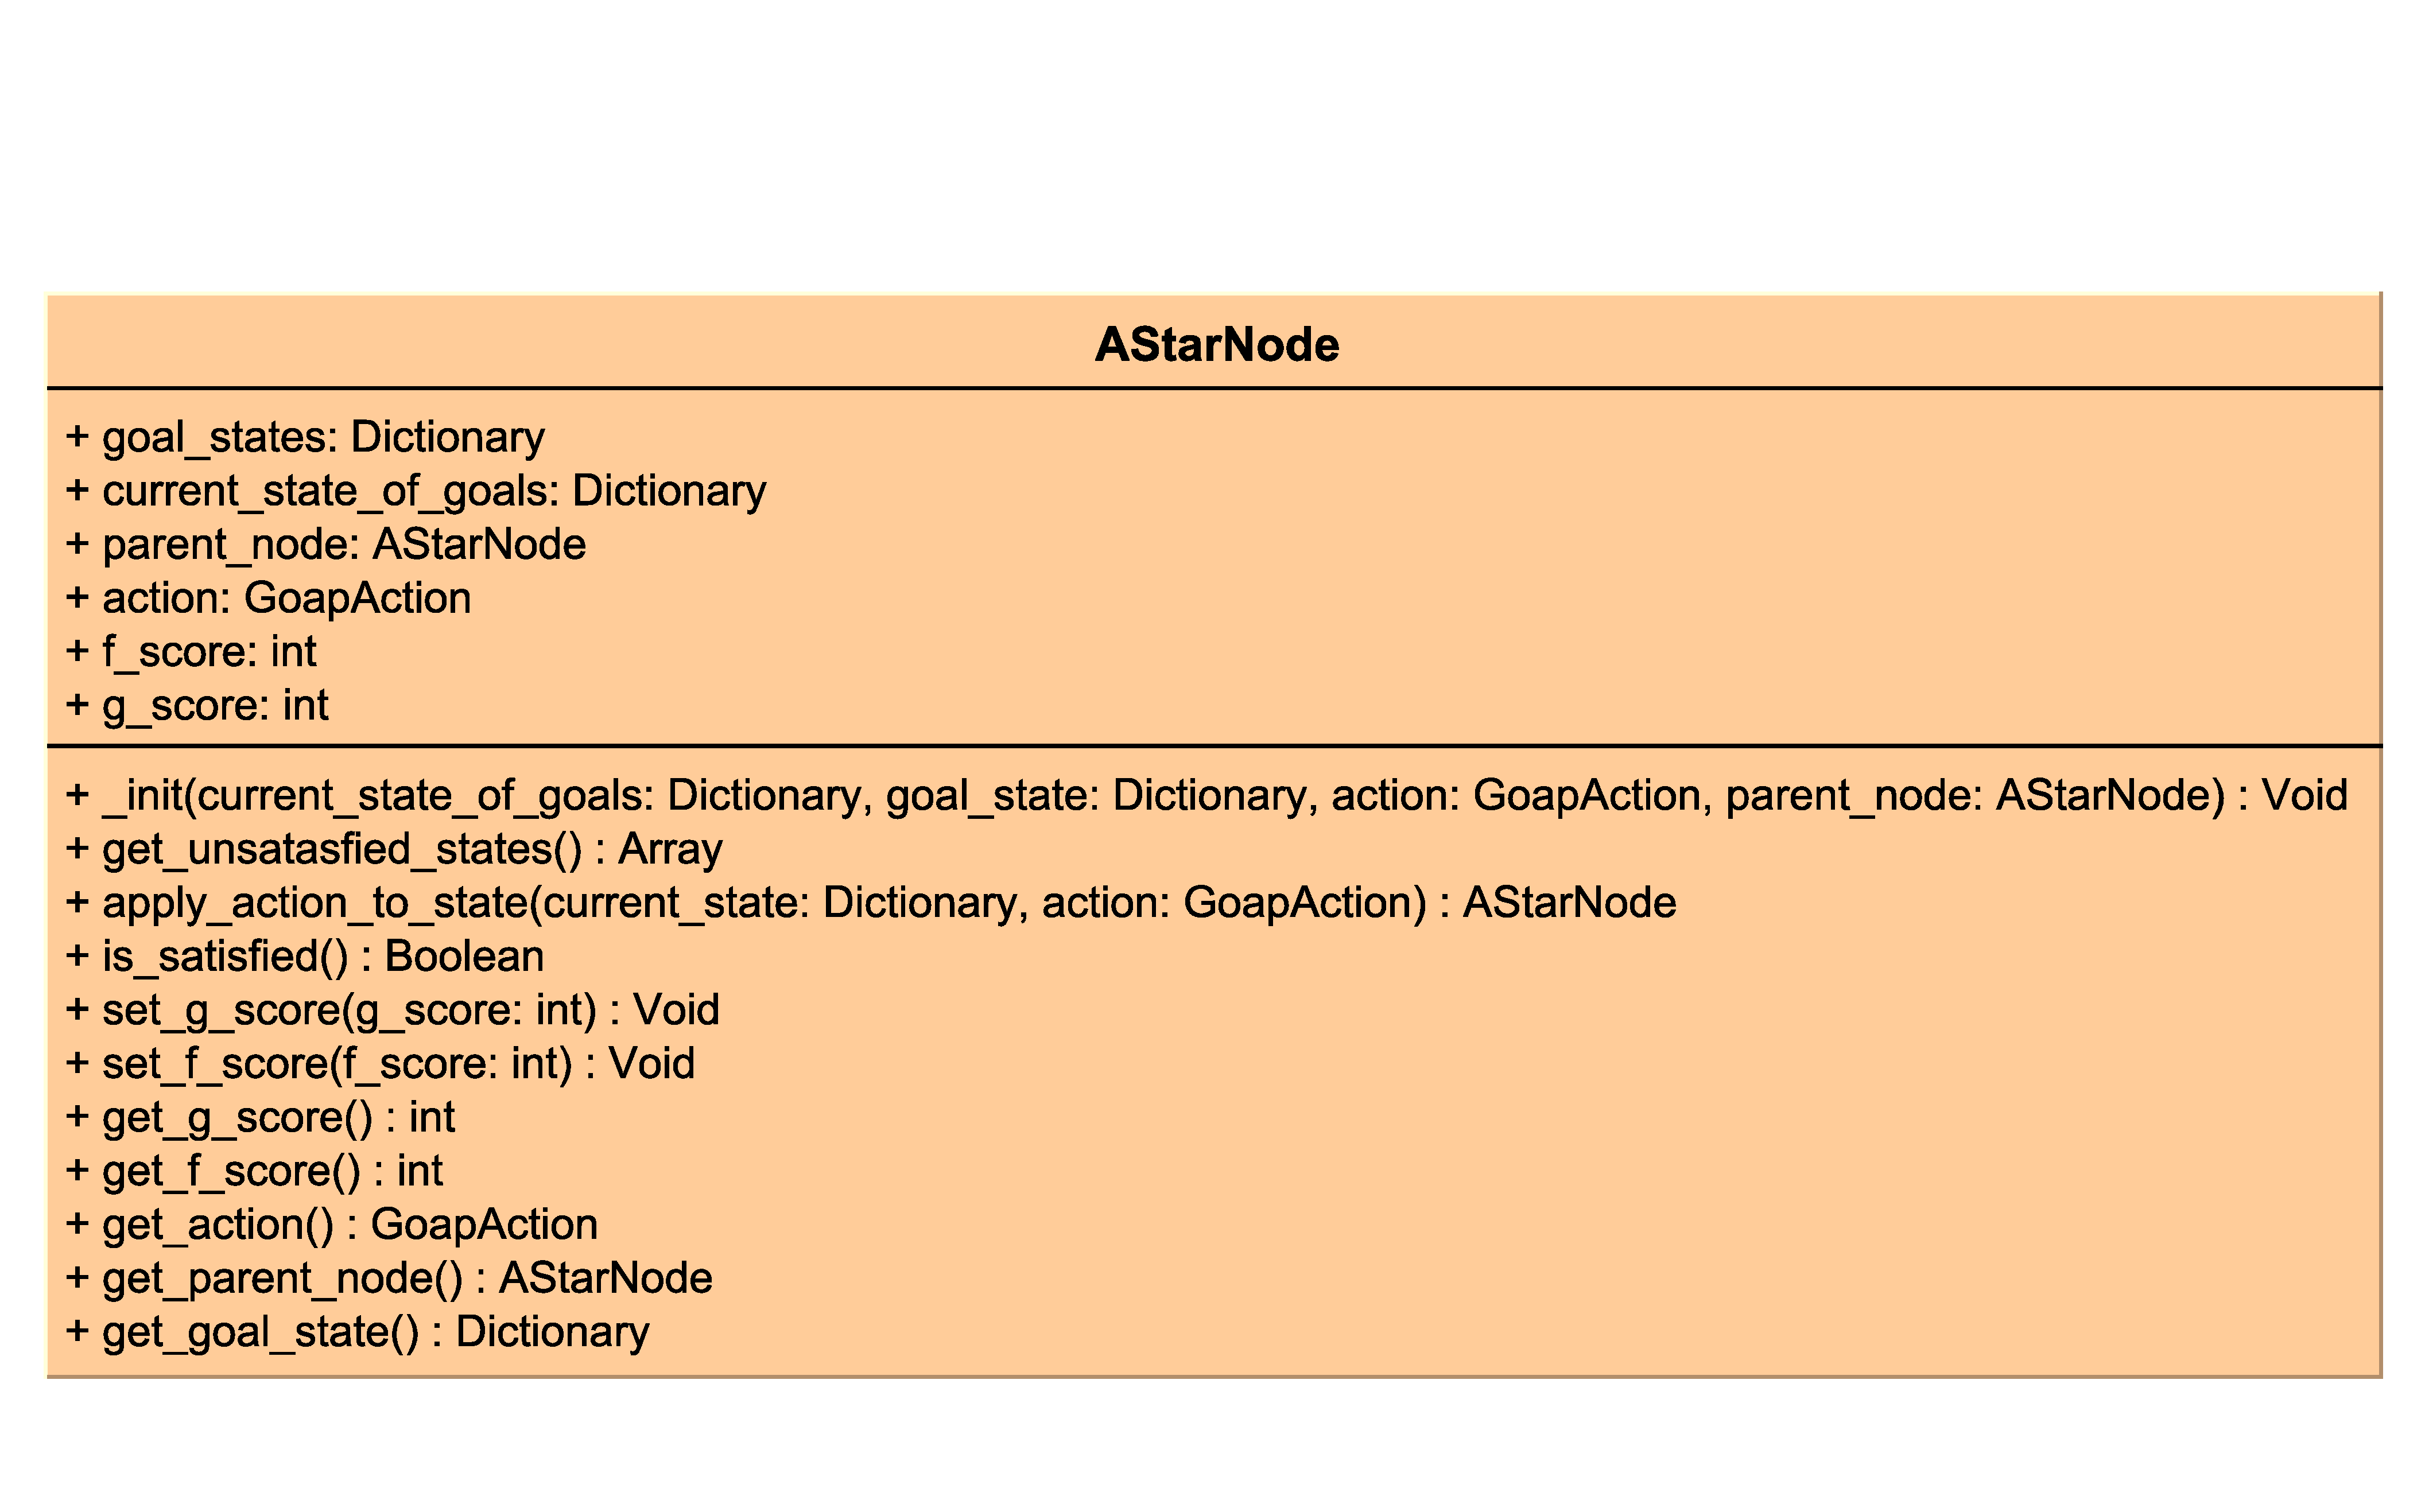
\includegraphics[width=0.9\textwidth, trim=20 20 20 20]{Lösungskonzept/astarnode.pdf}
	\captionsetup{justification=justified, format=plain}
  \caption{AStarNode}
  \label{fig:AStarNode}
\end{figure}


\subsubsection{Klassenattribute}
\label{chap:astarnode klassenattribute}

Ein AStarNode speichert die Informationen des Suchproblems. Darunter die bis dahin erfüllten Zustände des Elternknoten parent\_node im Attribut current\_state\_of\_goals, sowie alle Zielzustände die bis zu dem Knoten benötigt wurden im Attribut goal\_state. Über das Klassenattribut parent\_node kann die create\_path Methode des GoapPlanner rekursiv auf die Aktionen action des Typs GoapAction zurückschließen. Die Kosten $f(n)$ werden unter f\_cost und $g(n)$ -Kosten unter g\_cost gespeichert.


\subsubsection{Methoden}
\label{chap:astarnode methoden}

Durch den Godot Konstruktor \_init wird ein AStarNode mit seinen Attributen instanziiert. Die Berechnung der Kosten passiert durch die GoapPlanner Methode expand\_node. Dort werden über die setter- Methoden des AStarNode set\_g\_cost und set\_f\_cost initialisiert. Über die Methode get\_unsatasfied\_states werden alle Zustände zurückgegeben, welche noch nicht erreicht wurden. Die Größe des Arrays welches von get\_unsatasfied\_states gegeben wird repräsentiert die heuristischen Kosten $f(n)$ der Aktion. Die Heuristik Kosten werden ebenfalls in der expand\_node Methode des GoapPlanner berechnet und initialisiert.

Wird eine action gewählt, so wird ein AStarNode mit den dazugehörigen Zuständen current\_state\_of\_goals und goal\_states generiert werden. Die Generierung des neuen AStarNode geschieht über die apply\_action\_to\_state Methode. Die Methode wird vom GoapPlanner durch die Methode get\_child\_nodes auf dem expanded\_node aufgerufen. Dabei wird die action und der current\_state als Parameter übergeben. Basierend auf den Parameter initialisiert die Methode, die Attribute goal\_states und current\_state\_of\_goals für den neuen Knoten. Außerdem initialisiert sie den zu expandierten Knoten als parent\_node sowie die Aktion als action.

Die Prüfung ob die Zustände eines expanded\_node erfüllt wurden, wird durch is\_satasfied geprüft. Dazu schaut die Methode ob das Array welches über die Methode get\_unsatasfied\_states zurückgegeben wird leer ist. Sollte das Array leer sein, so gibt es keine zu erfüllenden Zustände und der AStarNode ist der Zielknoten.


\subsection{GoapGoal}
\label{chap:goapgoal uml}

Ein GoapGoal repräsentiert ein Ziel. Der GoapPlanner bewertet die verfügbaren Ziele, vergleicht sie miteinander und wählt eines aus, basierend auf deren Gültigkeit und Priorität. Der Zielzustand des jeweiligen GoapGoal wird als Ausgangszustand für Suche genutzt. Die Klasse GoapGoal wird in der folgenden Abbildung mittels UML-Notation dargestellt.

\begin{figure}[t]
  \centering
  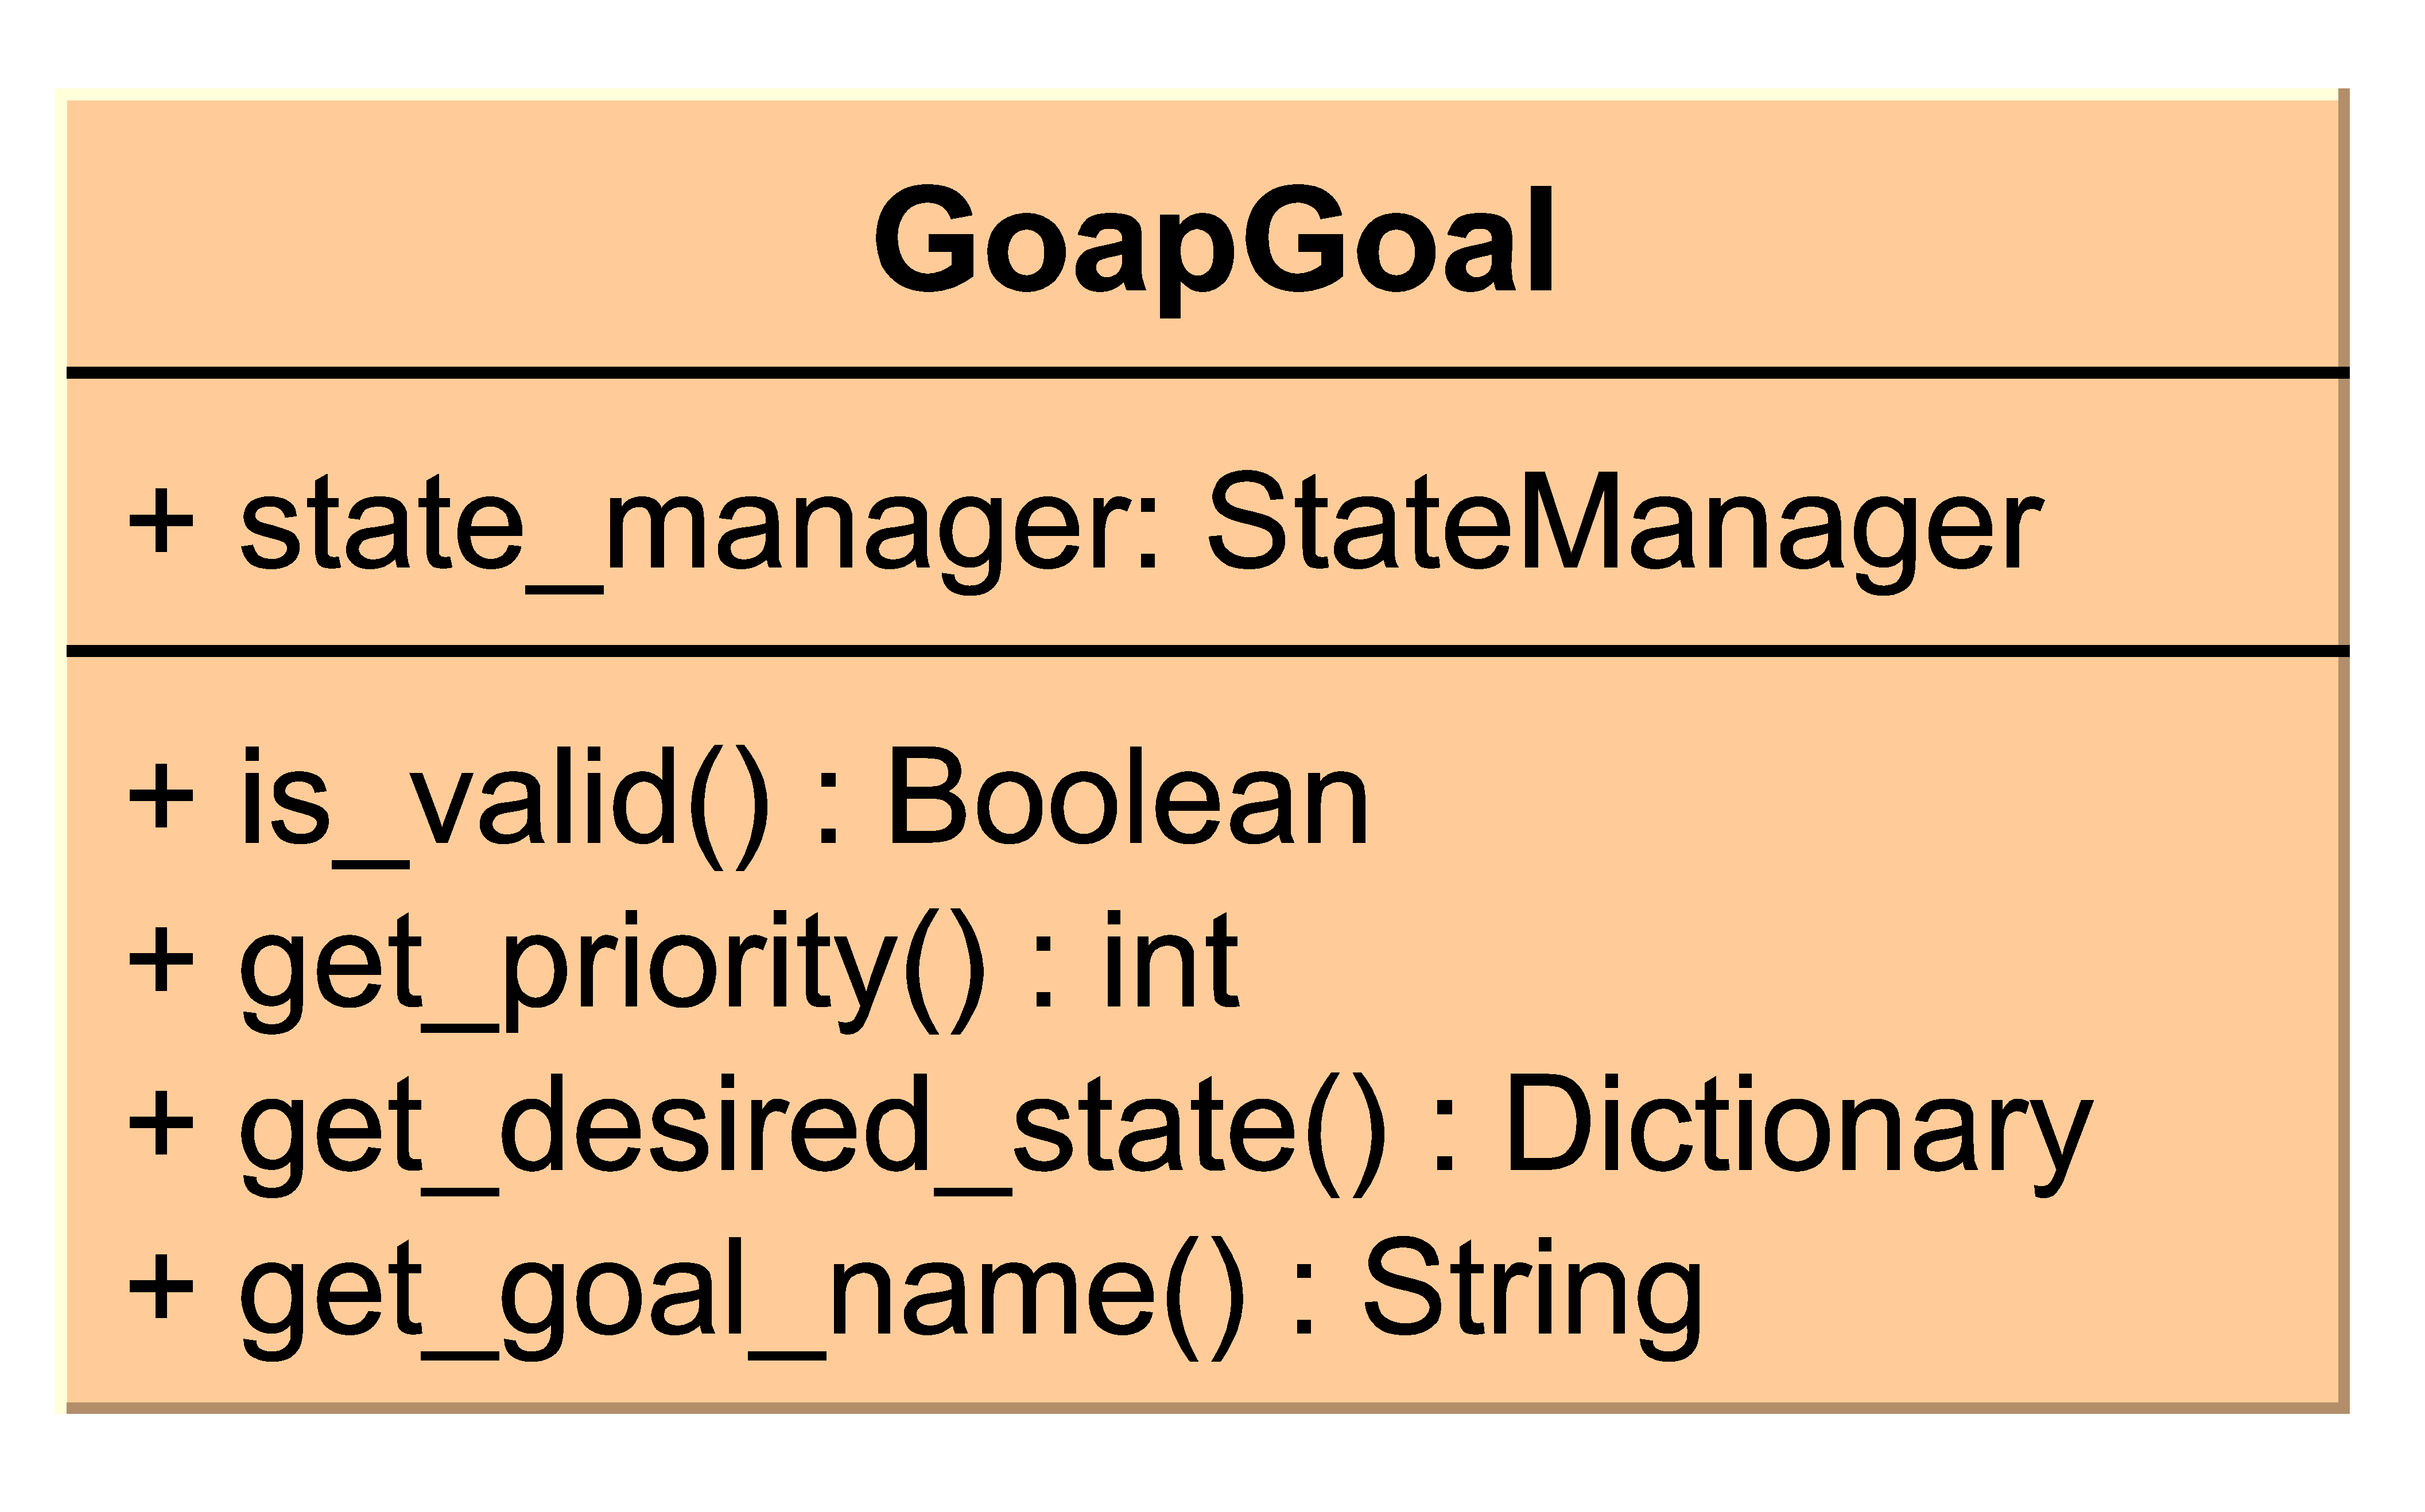
\includegraphics[width=0.5\textwidth, trim=20 20 20 20]{Lösungskonzept/goal.pdf}
	\captionsetup{justification=justified, format=plain}
  \caption{GoapGoal}
  \label{fig:GoapGoal}
\end{figure}

Die Priorität und Gültigkeit wird aus dem Klassenattribut state\_manager abgeleitet. Die get\_best\_goal des GoapPlanner benötigt die Gültigkeit und Priorität, um in folge dessen das Ziel auszuwählen. Die Abfragen geschehen durch die Methoden get\_priority und is\_valid. Ein Ziel wird erst dann berücksichtigt, wenn es durch die Methode is\_valid als gültig bestätigt wurde. Anschließend kann dessen Priorität mithilfe von get\_priority ermittelt werden. 

Über die Methode get\_desired\_state werden die Zielzustände aufgerufen, welche der GoapPlanner zur Suche der action\_sequence benötigt. 

Die Methode get\_goal\_name gibt den Klassennamen des GoapGoal zurück, welche von Debug Methoden genutzt werden kann.


%FORTSETZUNG
\subsection{GoapAction}
\label{chap:goapaction uml}

Ein Aktion des Typs GoapAction, repräsentieren die Kanten eines Suchbaums. Sie besitzen Daten zur Generierung eines neuen Knoten. Folgende Abbildung stellt die GoapAction Klasse nach UML-Notation dar.

\begin{figure}[h]
  \centering
  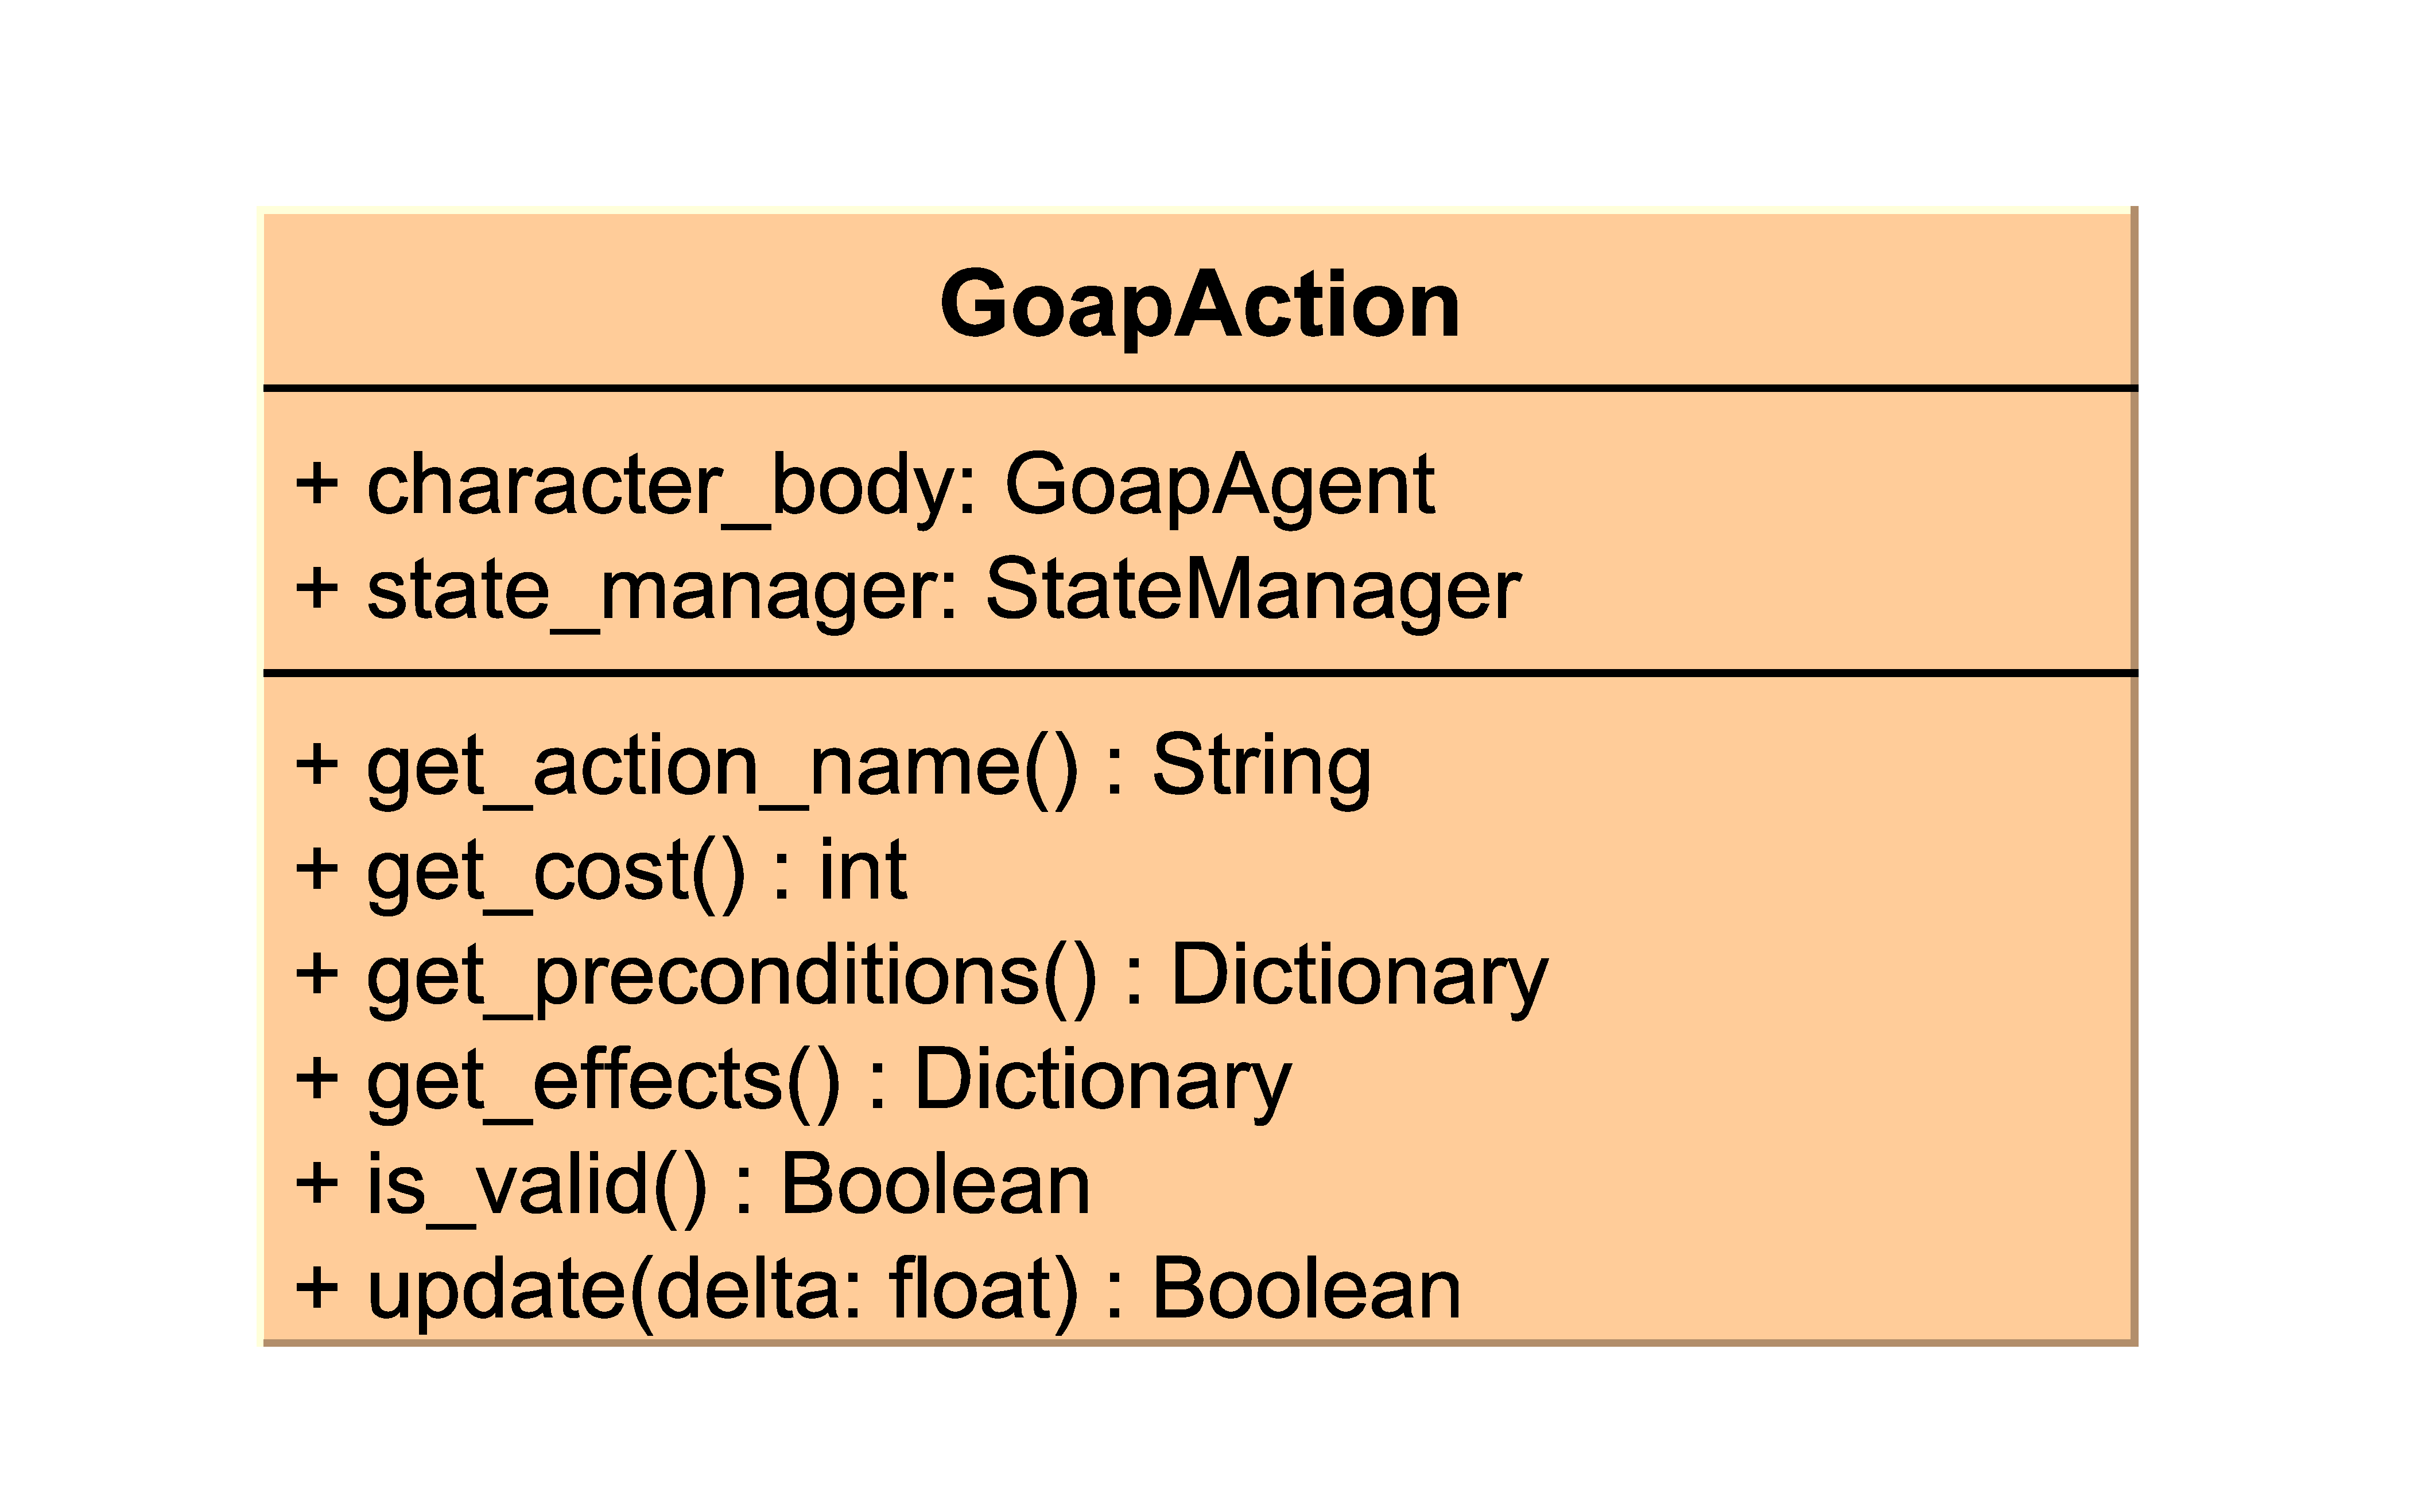
\includegraphics[width=0.7\textwidth, trim=20 20 20 20]{Lösungskonzept/action.pdf}
	\captionsetup{justification=justified, format=plain}
  \caption{GoapAction}
  \label{fig:GoapAction}
\end{figure}

Mit Hilfe der Klassenattribute character\_body und state\_manager werden die Kosten $g(n)$ und die Gültigkeit der Aktion gelesen. Die Kosten $g(n)$ werden dabei über die get\_cost Methode berechnet.

Die Gültigkeit einer Aktion soll die Durchführbarkeit wiedergeben. Der GoapPlanner wählt nur Aktionen aus, welche im derzeitigen Zustand des NPC durchführbar sind. Die Gültigkeit der Aktionen wird auch vor der Ausführung der update Methode jeweiligen Aktion durch den GoapAgent geprüft, da die Aktion zu einer Zeit ausgeführt werden kann in der sich der Zustand des NPC wieder ändern kann und somit auch die Gültigkeit. Für die Rückgabe der Gültigkeit ist die is\_valid Methode zuständig.

Eine get\_preconditions Methode gibt die vorausgesetzten Zustände zurück, welche von anderen Aktionen erfüllt werden müssten. Ob eine Aktion einen Zustand erfüllen kann, hängt von der get\_effects Methode ab, welche ein \textit{Dictionary} mit dem Zustand und dessen Wert zurückgibt. Stimmt der Wert des Zustands mit dem Zielzustand überein, dann erfüllt die Aktion den Zustand.

Die update Methode leitet die eigentliche Ausführung der Aktion ein und wird über den GoapAgent gestartet. Die Hoffnung dabei ist, dass die Aktion den erwünschten Wert des Effekts umsetzt. Aufgrund der nicht-deterministischen Natur der Spielwelt kann es jedoch vorkommen, dass der angestrebte Effekt nicht erreicht wird. Wird der Effekt nicht erreicht, so wird eine neue Sequenz angefordert oder das Ziel ändert sich bis dahin. Die Ausführung der Aktion wird dabei über \hyperref[chap:game-objects]{Komponenten} der Klasse Npc umgesetzt. Die Methode get\_action\_name gibt den Klassennamen der GoapAction zurück.


\section{Umsetzung des Szenario}
\label{chap:implementierung szenario}

Die Benchmarks benötigen eine Umgebung auf der die NPCs mit ihren jeweiligen Entscheidungssystemen getestet werden. Zu diesem Zweck agieren die NPCs\ref{} in einer 2D kartierbaren Spielwelt, die in der Abbildung \ref{} dargestellt wird. Die NPC-Klassen unterscheiden sich in ihren Entscheidungssystemen, die Komponenten, die für eine Ausführung einer Aktion benötigt werden bleiben für alle NPC Klassen identisch und werden mit der Oberklasse Npc vererbt. Bei den Komponenten handelt es sich um: Health-, Hit-, Melee-, Shoot-, Neighbor-, Move, LookAt-, Patrol-, Cover-, Vision- und PlayerBlock-Component. Sie ändern dabei die Zustände des StateManger, die in der GOAP Architektur erläutert wird\ref{}.

\begin{figure}[h]
  \centering
  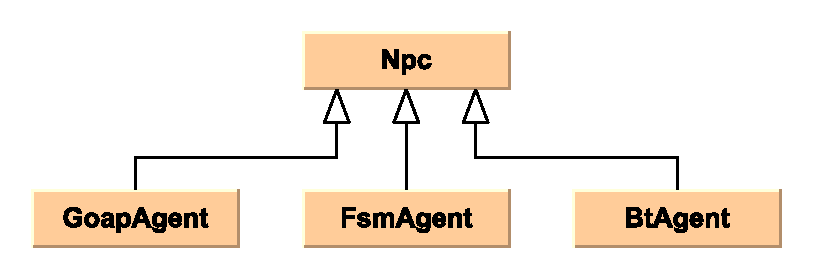
\includegraphics[width=0.7\textwidth, trim=20 20 20 20]{Implementation/npc class.pdf}
	\captionsetup{justification=justified, format=plain}
  \caption{Vererbung der Npc Klasse}
  \label{fig:npc class}
\end{figure}

\begin{figure}[h]
  \centering
  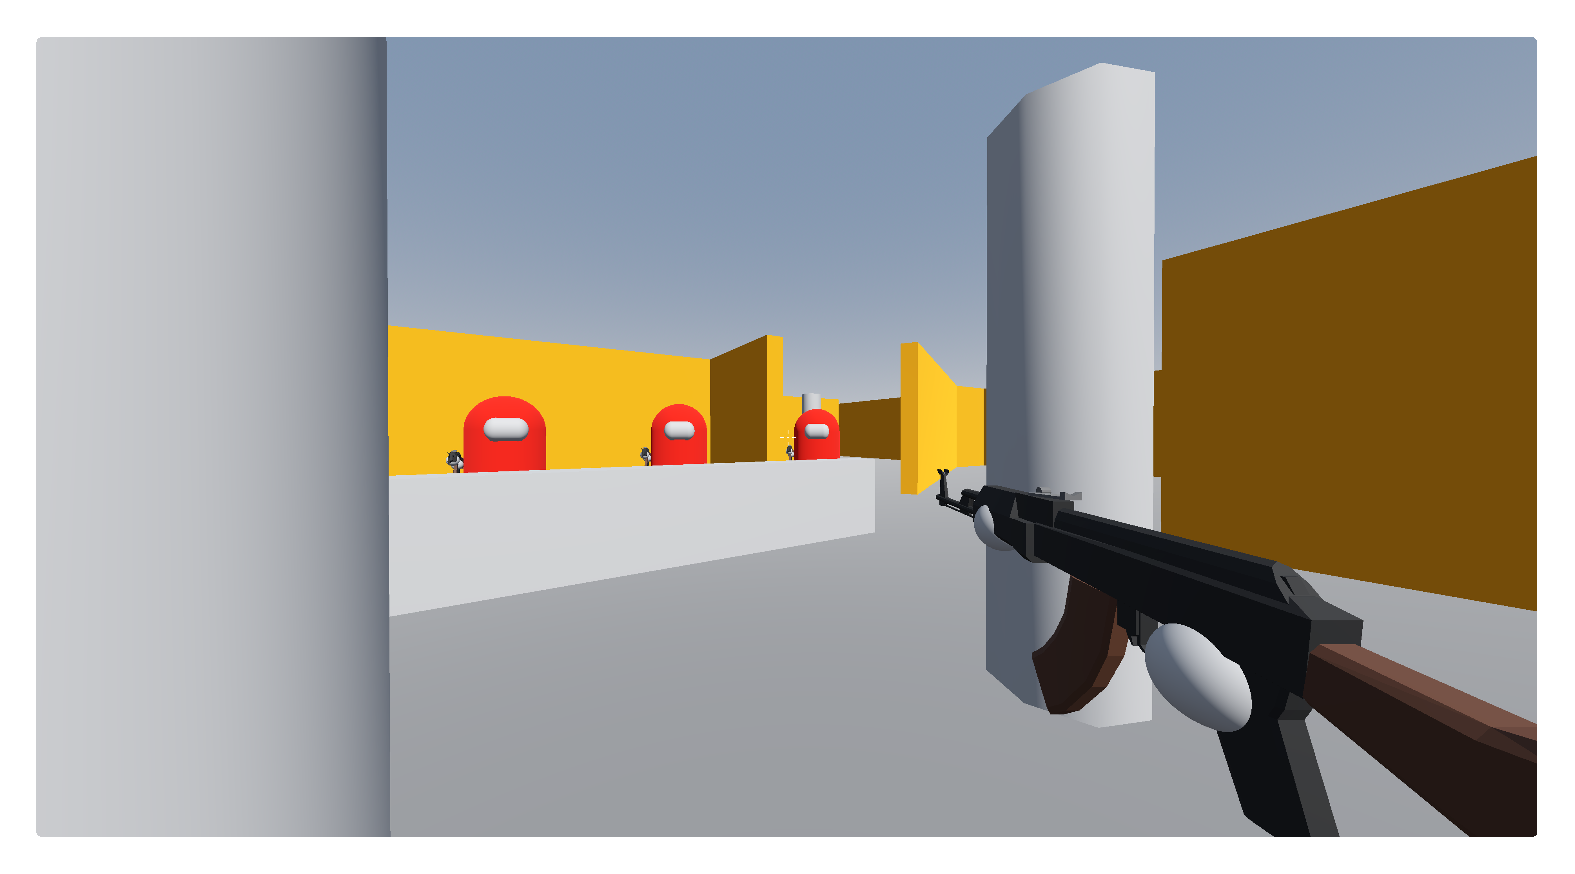
\includegraphics[width=0.7\textwidth, trim=20 20 20 20]{Implementation/ego shooter.pdf}
	\captionsetup{justification=justified, format=plain}
  \caption{Ego-Perspektive des Spieler und Spielwelt}
  \label{fig:ego shooter}
\end{figure}

Der Performance-Benchmark\ref{}, speichert während der Ausführung die Häufigkeit der Bilder-Pro-Sekunde für die jeweilige Anzahl an NPCs im gesamten Szenario. Der Benchmark beginnt mit einem NPC und wächst kontinuierlich, wobei alle 30 Sekunden ein neuer NPC der jeweiligen Klasse in die Spielwelt instanziiert wird. Für jede NPC-Klasse wird der Benchmark dreimal ausgeführt. Abschließend wird aus den gesammelten Daten der durchschnittliche FPS-Wert für jede NPC-Anzahl berechnet.

Der Speicher-Benchmark\ref{}, gibt den Speicherverbrauch des gesamten Szenario. Auch dieser Benchmark beginnt mit einem NPC und wächst kontinuierlich, wobei alle 10 Sekunden ein neuer NPC der jeweiligen Klasse in die Spielwelt instanziiert wird. Für jede NPC-Klasse wird der Benchmark einmal ausgeführt. Abschließend wird auch hier aus den gesammelten Daten der durchschnittliche Speicherverbrauch für jede NPC-Anzahl berechnet.
